% ****** Start of file apssamp.tex ******
%
%   This file is part of the APS files in the REVTeX 4.2 distribution.
%   Version 4.2a of REVTeX, December 2014
%
%   Copyright (c) 2014 The American Physical Society.
%
%   See the REVTeX 4 README file for restrictions and more information.
%
% TeX'ing this file requires that you have AMS-LaTeX 2.0 installed
% as well as the rest of the prerequisites for REVTeX 4.2
%
% See the REVTeX 4 README file
% It also requires running BibTeX. The commands are as follows:
%
%  1)  latex apssamp.tex
%  2)  bibtex apssamp
%  3)  latex apssamp.tex
%  4)  latex apssamp.tex
%
\documentclass[%
 reprint,
%superscriptaddress,
%groupedaddress,
%unsortedaddress,
%runinaddress,
%frontmatterverbose, 
%preprint,
%preprintnumbers,
%nofootinbib,
%nobibnotes,
%bibnotes,
 amsmath,amssymb,
 aps,
%pra,
%prb,
%rmp,
%prstab,
%prstper,
%floatfix,
]{revtex4-2}
\usepackage{kotex}
\usepackage{graphicx}% Include figure files
\usepackage{dcolumn}% Align table columns on decimal point
\usepackage{bm}% bold math
\usepackage{tikz}
\usetikzlibrary{arrows}

% Nice captions.
\usepackage[hang,small,bf]{caption}
\setlength{\captionmargin}{25pt}

% New commands to keep things tidy.

%\usepackage{hyperref}% add hypertext capabilities
%\usepackage[mathlines]{lineno}% Enable numbering of text and display math
%\linenumbers\relax % Commence numbering lines

%\usepackage[showframe,%Uncomment any one of the following lines to test 
%%scale=0.7, marginratio={1:1, 2:3}, ignoreall,% default settings
%%text={7in,10in},centering,
%%margin=1.5in,
%%total={6.5in,8.75in}, top=1.2in, left=0.9in, includefoot,
%%height=10in,a5paper,hmargin={3cm,0.8in},
%]{geometry}

\def\rcurs{{\mbox{$\resizebox{.16in}{.08in}{
\includegraphics{ScriptR}}$}}}
\def\brcurs{{\mbox{$\resizebox{.16in}{.08in}{
\includegraphics{BoldR}}$}}}
\def\hrcurs{{\mbox{$\hat \brcurs$}}}

\begin{document}


\title{리드베리 상수 측정 실험 보고서}

\author{서울대학교 전기정보공학부 2018-12432 박정현}
 \email{alexist@snu.ac.kr}
\date{실험일 : 10/16/2023, 제출일: \today}% It is always \today, today,
             %  but any date may be explicitly specified

\begin{abstract}
본 실험에서는 수소와 수은 방전관으로부터 스펙트럼을 측정하여 리드베리 상수를 측정하고 측정된 power와 linewidth를 이론적으로 예측한 결과와 비교하였다. 이론적인 예측값과 대부분의 결과가 consistent함을 확인하였으며 그외의 오차는 boltzman factor와 다른 decay에 의한 것으로 결론지었다. 더 정확한 실험을 수행하기 위한 실험 방법 또한 제시하였다.
\end{abstract}

%\keywords{Suggested keywords}%Use showkeys class option if keyword
                              %display desired
\maketitle

%\tableofcontents

\section{\label{sec:level1}Introudction}
\subsection{\label{sec:level2}방전관}
유전체 양단에 강한 전압을 인가하면 전자들이 가속하여 원자들에 충돌하는 현상이 나타난다. 전자가 충돌한 원자는 다시 전자를 방출하고 electron avlanche가 발생하여 towndown discharge가 발생한다.  이때 방전관 내부에 있는 원자들이 전자들을 흡수, 방출하면서 방전관 외부로 광자를 방출하게 된다. 이 때 광자는 아래와 같이 원자들의 에너지 준위 차이에 해당하는 주파수를 가진다. 이러한 주파수, 혹은 파장에 따른 스펙트럼을 확인하면 원자의 에너지 준위를 분석할 수 있다.[2]

\begin{align}
	\frac{1}{\lambda} &= R\left(\frac{1}{n^{2}}-\frac{1}{m^{2}}\right)	\label{eq:rydbery}
\end{align}

\subsection{\label{sec:level2}스펙트럼}
원자 내부에는 다양한 에너지 레벨이 존재한다. 이러한 에너지 레벨이 충분히 멀리 떨어져 있는 경고 입사하는 광자의 에너지가 해당 에너지레벨 차이에 가까운 경우 2 level system으로 근사할 수 있다. Ground state, 그리고 상호작용하는 enery level을 모두 고려하면 Fig.\label{fig:Level}과 같이 에너지 레벨을 나타낼 수 있다. 이 때 외부로부터 excite되는 원자들의 비율이 $\Lambda$라고 할 때 아래의 식이 성립한다. 단, $\rho_{nm}$은 photon state $nm$에 대한 density matrix에 해당한다.

\begin{figure}
\centerline{
  \resizebox{8cm}{!}{
    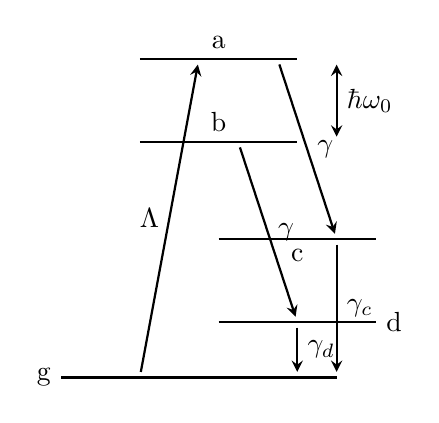
\begin{tikzpicture}[
      scale=0.5,
      level/.style={thick},
      virtual/.style={thick,densely dashed},
      trans/.style={thick,->,shorten >=2pt,shorten <=2pt,>=stealth},
      trans2/.style={thick,<->,shorten >=2pt,shorten <=2pt,>=stealth},
      classical/.style={thin,double,<->,shorten >=4pt,shorten <=4pt,>=stealth}
    ]
    % Draw the energy levels.
    \draw[level] (6cm,-12em) -- (-1cm,-12em) node[left] {g};
    \draw[level] (1cm,11em) -- (5cm,11em) node[midway,above] {a};
    \draw[level] (3cm,-8em) -- (7cm,-8em) node[right] {d};
    % Draw the virtual levels.
    \draw[level] (1cm,5em) -- (5cm,5em) node[midway,above] {b};
    \draw[level] (3cm,-2em) -- (7cm,-2em) node[midway,below] {c};
    % Draw the transitions.
    \draw[trans] (1cm,-12em) -- (2.5cm,11em) node[midway,left] {$\Lambda$};
    \draw[trans2] (6cm,5em) -- (6cm,11em) node[midway,right] {$\hbar \omega_{0}$};
    \draw[trans] (3.5cm,5em) -- (5cm,-8em) node[midway,right] {$\gamma$};
    \draw[trans] (4.5cm,11em) -- (6cm,-2em) node[midway,right] {$\gamma$};
    \draw[trans] (5cm,-8em) -- (5cm,-12em) node[midway,right] {$\gamma_{d}$};
    \draw[trans] (6cm,-2em) -- (6cm,-12em) node[midway,right] {$\gamma_{c}$};
    \end{tikzpicture}
  }
}
\caption{\label{fig:Level}방전관에서 광자 방출 diagram}
\end{figure}

\begin{align}
	\dot{\rho}_{nm} &= -\frac{i}{\hbar}\text{Tr}_{atom}[H_{I},\rho]_{nm} + (L\rho)_{nm}
\end{align}

위의 식을 정리하면 아래와 같아진다.

\begin{align}
	\begin{split}
	\dot{\rho}_{nm} &= -\left(\frac{N_{nm}'G}{1+N_{nm}S/G}\right)\rho_{nm} \\
	& + \left(\frac{\sqrt{nm} G}{1+N_{n-1,m-1}S/G}\right)\rho_{n-1,m-1} \\
	& - \kappa(n+m)\rho_{nm} \\
	& + 2\kappa\sqrt{(n+1)(n+1)}\rho_{(n+1)(m+1)}
	\end{split}
\end{align}

단, 상수들은 아래와 같다.

\begin{align}
	G &= N\frac{\Lambda}{\gamma + \Lambda} \frac{2g^{2}}{\gamma} \\
	S &= \frac{4g^{2}}{\gamma^{2}}G\\
	N_{nm}' &= \frac{1}{2}(n+1+m+1) + \frac{(n-m)^{2}S}{8G}\\
	N_{nm} &= \frac{1}{2}(n+1+m+1) + \frac{(n-m)^{2}S}{16G}
\end{align}

$n=m$인 경우만 고려하면 $\rho_{nm} = p(n)$에 해당한다. $S\langle n \rangle / G \gg 1$이고 pumping rate가 충분히 커 $\Lambda \gg \gamma $인 경우를 고려하면 평균 광자수 $\langle n \rangle$ 은 아래와 같아진다.
\begin{align}
	\langle n \rangle &\simeq \frac{G}{2\kappa}\left( \frac{G-2\kappa}{S} \right)\\
	&\simeq N\frac{\Lambda}{\gamma + \Lambda} \frac{2g^{2}}{2\kappa\gamma} \frac{\gamma^{2}}{4g^{2}}\\
	& \simeq N\frac{\gamma}{4\kappa}
\end{align}

광자의 방출을 random event로 고려하는 경우 line width는 아래와 같아진다.

\begin{align}
	\Delta \omega \simeq \frac{2\kappa}{\langle n \rangle}\label{eq:final_linewidth}
\end{align}

Spontaneous decay rate만을 고려하면 $\gamma$는 아래와 같아진다.

\begin{align}
	\gamma \simeq \frac{2e^{2}\omega_{0}^{2}}{3mc^{2}}
\end{align}

따라서 에너지 사이의 간격 $\omega_{0}$가 커지는 경우 $\gamma$가 증가하므로 평균 광자수가 증가한다. 또한 평균 광자수가 증가하므로 line width는 이에 비례하여 작아지게 된다.[1] 이 때 열적 평형 상태에 있는 경우 각 state의 비율은 볼츠만 factor를 곱한 값과 같고 최종적으로 측정되는 power는 아래와 같다. 작은 주파수 대역에서는 power가 증가하고 큰 주파수에서는 감소하는 형태를 띨것을 알 수 있다. 
\begin{align}
	P &= \langle n \rangle\exp\left(-\frac{\hbar\omega_{0}}{kT}\right)\label{eq:finalpower}
\end{align}


\section{\label{sec:level1}Data\&Results}
\subsection{\label{sec:level2}수소}
수소 스펙트럼 측정 결과는 Figs.\ref{fig:Hydrogen1}, \ref{fig:Hydrogen2}와 같다. 단, Fig.\ref{fig:Hydrogen1}, 300ms의 exposure time을 가지고 측정한 결과이며, Fig.\ref{fig:Hydrogen2}는 $30ms$의 exposure time을 가지고 측정한 결과이다. 300ms의 exposure time을 가지는 경우 656nm에서 최대 측정 power의 범위를 넘어가 30ms에서 추가적으로 측정하였다. 또한 각각의 peak에서 linewidth와 frequency를 측정하기 위해 각각의 peak에서 gaussian function에 대해서 fitting을 수행하였다. 이를 통해 측정한 파장은 Tab.\ref{tab:lambda}와 같다. 모두 $1\%$미만의 오차를 가진다. 

\begin{figure}[htbp]
	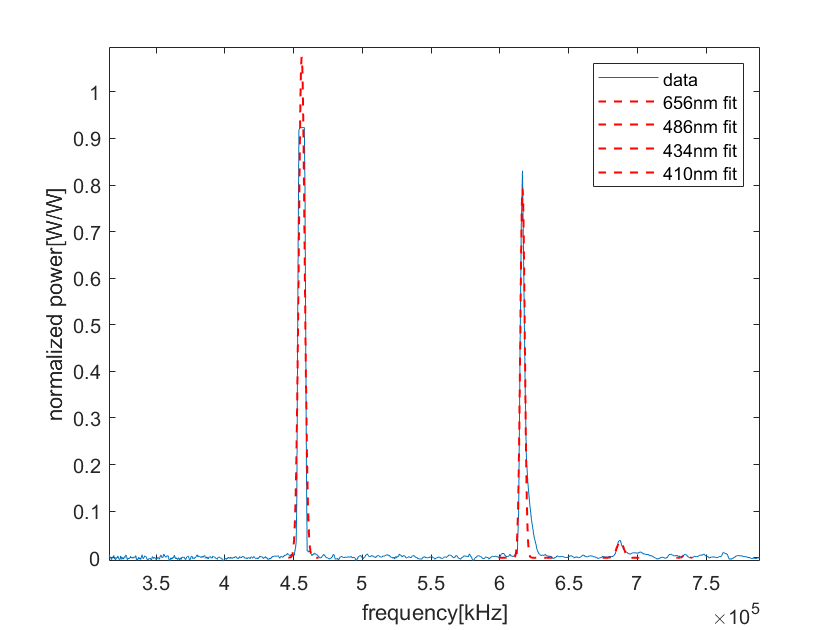
\includegraphics[width = 0.95\linewidth]{Hydrogen1.png}% Here is how to import EPS art
	\caption{\label{fig:Hydrogen1}수소의 방출 스펙트럼 with 300ms exposure time}
\end{figure}

\begin{figure}[htbp]
	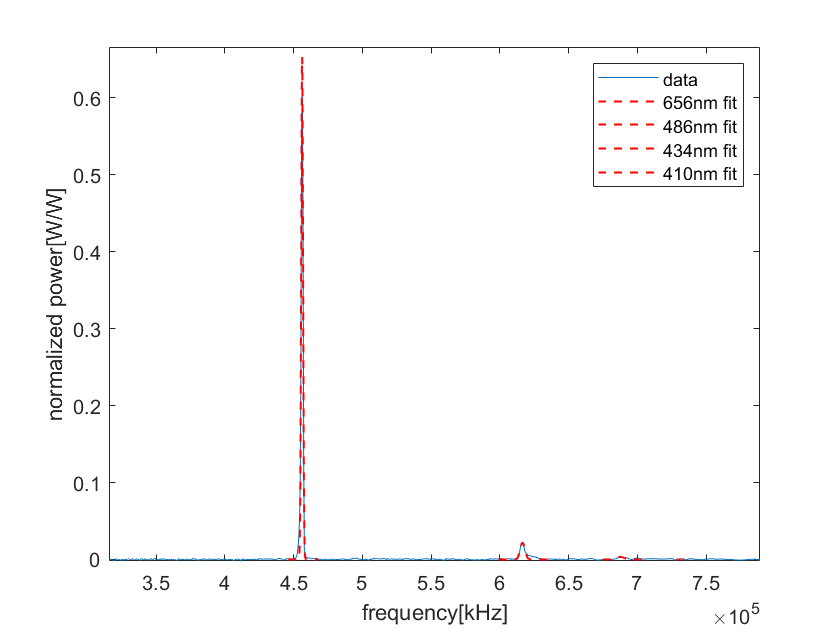
\includegraphics[width = 0.95\linewidth]{Hydrogen2.png}% Here is how to import EPS art
	\caption{\label{fig:Hydrogen2}수소의 방출 스펙트럼 with 30ms exposure time}
\end{figure}

\begin{table}[]
\begin{tabular}{c|c|c} \hline \hline
전자전이 & 측정값[nm] & 오차 \\ \hline
$3\rightarrow 2$& 657.97 & $0.26\%$\\ \hline
$4\rightarrow 2$& 486.58 & $0.092\%$\\ \hline
$5\rightarrow 2$& 436.30 & $0.52\%$\\ \hline
$6\rightarrow 2$& 408.20 & $0.48\%$\\ \hline
\end{tabular}
\caption{\label{tab:lambda}수소 스펙트럼 측정 결과}
\end{table}

측정 결과를 식 (\ref{eq:rydbery})에 fitting한 결과는 Fig.\ref{fig:Rydbery}와 같다. 이를 이용해 리드베리 상수를 계산하면 식(\ref{eq:ryd_val})와 같다. 알려진 리드베리 상수 $1.097\times 10^{7}[m^{-1}]$와 비교했을 때 $0.8\%$의 오차를 가진다.[2]

\begin{align}
	R &= (1.11\pm0.03)\times 10^{7}[m^{-1}]\label{eq:ryd_val}
\end{align}

\begin{figure}[htbp]
	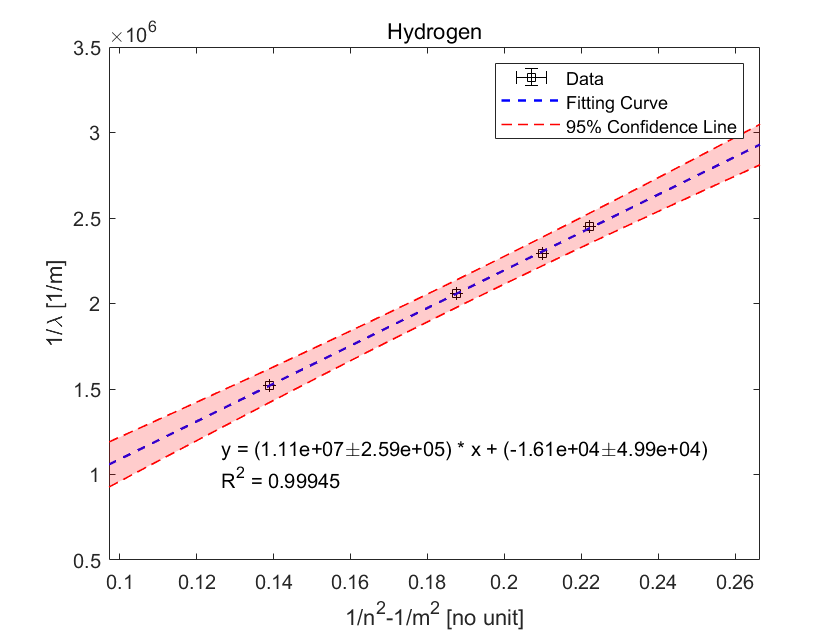
\includegraphics[width = 0.95\linewidth]{Rydbery.png}% Here is how to import EPS art
	\caption{\label{fig:Rydbery}Peak fitting 결과}
\end{figure}

각 피크별 amplitude와 linewidth 측정 결과는 Fig.\ref{fig:Hydrogen2}을 gaussian function으로 fitting하여 계산하였으며 결과는 Tab.\ref{tab:linewidth}와 같다. 발머대역에서의 주파수 차이가 충분히 크므로 주파수가 커짐에 따라 $A$가 커지고 $\Delta \omega$가 감소하여 각각 (\ref{eq:finalpower}), (\ref{eq:final_linewidth})에서 예상한 이론적인 예측과 일치함을 알 수 있다. 하지만 측정된 power의 amplitude와 $\Delta \omega$의 곱이 상수가 아니며 주파수가 증가함에 따라 감소한다.

\begin{table}[]
\begin{tabular}{c|c|c|c} \hline \hline
전자전이 & $\Delta \omega$ [kHz] & A [A.U] & $A \Delta\omega [Hz]$ \\ \hline
$3\rightarrow 2$& 0.953 & 0.654 & $624$\\ \hline
$4\rightarrow 2$& 2.43 & 0.0219 & $53.3$\\ \hline
$5\rightarrow 2$& 3.81 & 0.0033 & $12.7$\\ \hline
$6\rightarrow 2$& 5.90 & 0.000542 & $3.20$\\ \hline
\end{tabular}
\caption{\label{tab:linewidth}수소 스펙트럼 peak 별 linewidth}
\end{table}


\subsection{\label{sec:level2}수은}
수은의 스펙트럼은 Fig.\ref{fig:Mercury}와 같다. (\ref{eq:finalpower})에서 예상한 형태와 consistent하다.
\begin{figure}[htbp]
	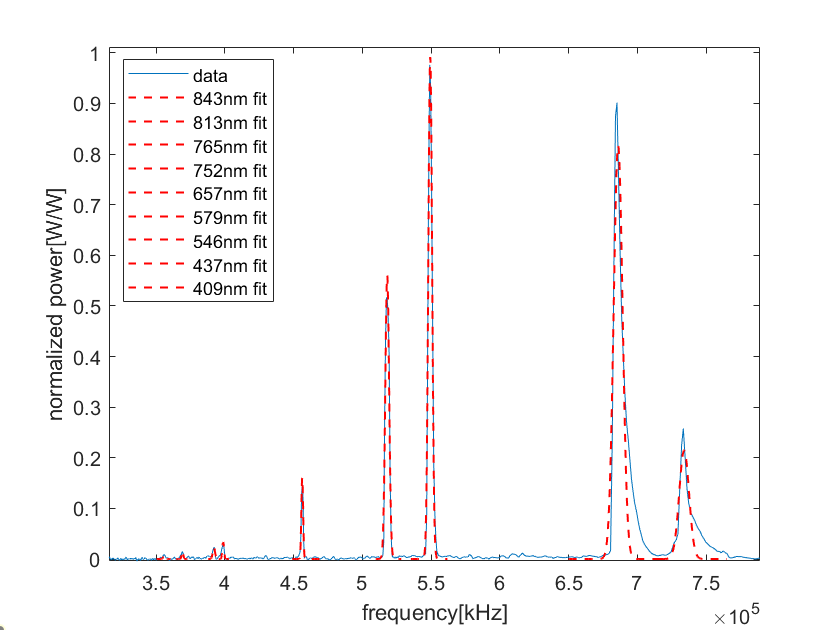
\includegraphics[width = 0.95\linewidth]{Mercury.png}% Here is how to import EPS art
	\caption{\label{fig:Mercury}수은 스펙트럼 결과}
\end{figure}


\section{\label{sec:level1}Conclusion\&Discussion}
주어진 실험결과는 모두 이론적 예상과 기대했던 값과 높은 재현도, 정확도에서 consistent하다. 하지만 수소 스펙트럼 결과에서 lienwidth와 output power의 곱은 일정하지 않았다. 이것은 boltzman factor에 의한 효과에 의한 것으로 결론지었다. 또한 linewidth의 경우 정확히 주파수의 제곱에 비례하지 않는데 이것은 decay가 spontaneous decay에만 의존할 뿐만 아니라 purcell effect, non radiative decay, collision 등 여러 요인에 의해 decay가 발생하기 때문에 발생한 것으로 결론지었다. 방전관이 아닌 hydrogen ion trap을 제작하여 스펙트럼을 측정하는 경우 더 정확한 값을 측정할 수 있을 것이다. 방전관을 이용하는 경우 더 높은 power를 측정할 수 있는 장비를 이용해 높은 exposure time에서 측정하고 완전한 암실에서 측정하는 경우 더 정확한 값을 측정할 수 있을 것이다.

\section{\label{sec:level1}Reference}

[1] Scully, M. O., S., \& Zubairy, M. S. (1997, September 4). \textit{Quantum Optics}. Cambridge University Press.

[2] Halliday, D., Resnick, R., \& Walker, J. (2013, August 5). \textit{Fundamentals of Physics}. Wiley.

\end{document}
%
% ****** End of file apssamp.tex ******
